\section{Design}\label{sec:design}

\sys{} has three parts: a capture library preloaded into the unmodified engine, a memory map
exported by the engine once, and an offline analysis that joins the two
(\cref{fig:pipeline}). The capture library is 350 lines of C++ against CUPTI; the memory map
exporter for vLLM is 60 lines of Python; the analysis is 330 lines of Python.

\begin{figure}[t]
\centering
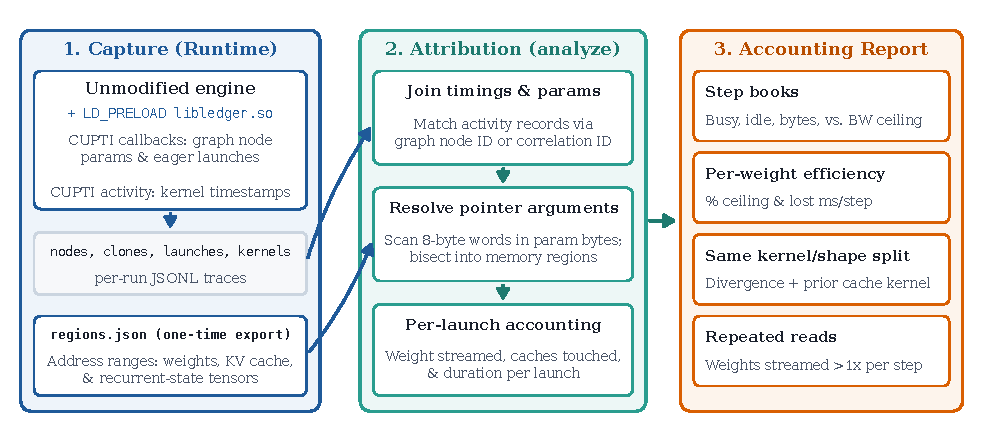
\includegraphics[width=\linewidth]{figures/pipeline}
\caption{\sys{} pipeline. The capture library runs inside the unmodified engine; attribution and reporting run offline.}\label{fig:pipeline}
\end{figure}

\subsection{Capture}\label{sec:capture}

\paragraph{What is recorded.}
For every kernel launch we want the function, the launch geometry, the raw bytes of every
parameter, and the start and end timestamps. Timestamps come from the CUPTI activity API
(concurrent-kernel records). Parameters are not part of activity records, so the library also
subscribes to CUPTI callbacks and copies them at launch time. A serving engine issues almost all
of its decode work through CUDA graphs: in our case study 927 of 972 launches per step. Graph replays do not pass through any launch API, so the parameters of graph
kernels must be taken when the graph is built.

\paragraph{CUDA graphs.}
On the \texttt{GRAPHEXEC\_CREATED} resource callback the library walks the nodes of the source
graph and records, for each kernel node, its function, geometry and parameter bytes
(via \texttt{cuGraph\-Kernel\-Node\-Get\-Params}) under its CUPTI graph node id. Instantiation clones nodes;
the \texttt{GRAPHNODE\_CLONED} callback records the clone-to-original mapping. An activity record
of a replayed kernel carries the id of the executable node, which the analysis maps back through
the clone chain to the recorded node.

\paragraph{Direct launches.}
Inside the profiling range the library also intercepts driver launches
(\texttt{cuLaunchKernel}, \texttt{cuLaunchKernelEx}) and runtime launches
(\texttt{cudaLaunchKernel}, \texttt{cudaLaunchKernelExC}) and records them under the CUPTI
correlation id, which the activity record carries as well.

\paragraph{Parameter layouts.}
The kernel parameter array is an array of pointers to arguments; copying it requires the offset
and size of each argument. The library queries them with \texttt{cuFuncGetParamInfo} and caches
the layout per \texttt{CUfunction}. Caching by kernel name is not safe: JIT compilers such as
Triton reuse a kernel name across modules with different signatures, and an early version of the
library that cached by name crashed the engine. A runtime launch names a host stub rather than a
function; the library resolves it through \texttt{cudaGetFuncBySymbol} of the cudart the
application already loaded (looked up with \texttt{RTLD\_NOLOAD}, since Python extensions load
cudart privately). A failed lookup leaves an error in cudart's per-thread last-error slot, which
the application would later report as its own, so the library clears it. For some runtime launches this lookup fails and CUPTI reports no symbol name; for those the library
falls back to a by-name layout found from the host stub, but only for names that have a single
layout everywhere in the process.

\paragraph{Window.}
Kernel timing is enabled between \texttt{cudaProfilerStart} and \texttt{cudaProfilerStop}, the
same convention Nsight Systems uses, so the engine is bracketed around a steady-state decode
window after warm-up and graph capture.

\subsection{Memory map}\label{sec:regions}

The analysis needs to know what each address is. The engine writes, once, a list of regions
\texttt{\{kind, name, addr, size, shape, dtype\}}. For vLLM the exporter runs in the worker via
\texttt{collective\_rpc} and lists every parameter and buffer of the model, every parameter of the draft model,
and every KV-cache and recurrent-state tensor from the static forward context, each with the
address range of its storage. In the case study this is 1779 regions. Activations and workspaces
are not listed.

\subsection{Attribution}\label{sec:attribution}

For each timed launch the analysis scans every 8-byte word of its parameter bytes and looks the
value up in the sorted region list. Words that hit a region are pointer candidates. A word that
equals the base of a region is trusted over one that lands inside a region, because interior hits
are often strides or packed fields. Of the weight regions a launch references, it is taken to
\emph{stream} the largest one, together with the tensors of the same module (quantization scales);
other weight hits are incidental. A launch too short to have read its weight at 1.3 times the
measured ceiling only gathered from it (an embedding lookup) and is counted as a partial read.
Cache regions referenced by a launch are recorded as \emph{touched}.

The byte model is deliberately simple: a weight-streaming launch reads its weight once. This holds
for decode with a handful of tokens per step, where activations are a small fraction of the
traffic, and fails for prefill and large batches (\cref{sec:limits}).

\subsection{Analysis}\label{sec:analysis}

The report has four parts.

\paragraph{Step books.} Wall time, GPU busy time (union of kernel intervals), idle time between
kernels, launches, weight bytes streamed, effective bandwidth, and the floor: the step time if
every byte moved at the measured ceiling.

\paragraph{Per-weight efficiency.} Launches are grouped by the weight they stream, with the layer
index folded (\texttt{layers.N}), shape and dtype. For each group the report gives the bandwidth
achieved and the time lost per step against the ceiling, sorted by time lost.

\paragraph{Same kernel, same shape, different speed.} Launches of one kernel with the same grid on
weights of the same shape and dtype read the same number of bytes with the same code. If their
durations split by weight group, by more than 15\% in the median, the difference comes from the
surroundings rather than from the kernel. For each such split the report gives the excess per
launch and per step, and for each side the most frequent kernel, among the three launches before it, that last touched a
cache region. That kernel is the suspect: its writes are the ones most likely to still be in L2.

\paragraph{Repeated reads.} Weights streamed more than once per step, with the extra bytes.

These checks encode invariants rather than models of the hardware: the same bytes through the
same code should cost the same; a weight should be read once per step. A violation does not say
why; it says where to run a controlled experiment (\cref{sec:case}).
